%%%%%%%%%%%%%%%%%%%%%%%%%%%%%%%%%%%%%%%%%%%%%%%%%%%%%%%%%%%%%%%%%%%%%
% LaTeX Template: Project Titlepage Modified (v 0.1) by rcx
%% Original Source: http://www.howtotex.com

\documentclass[12pt]{report}
\usepackage[a4paper]{geometry}
\usepackage[myheadings]{fullpage}
\usepackage{fancyhdr}
\usepackage{lastpage}
\usepackage{graphicx, wrapfig, subcaption, setspace, booktabs}
\usepackage[T1]{fontenc}
\usepackage[font=small, labelfont=bf]{caption}
\usepackage{fourier}
\usepackage{titlepic}
\usepackage[protrusion=true, expansion=true]{microtype}
\usepackage[english]{babel}
\usepackage{sectsty}
\usepackage{url, lipsum}
\usepackage{hyperref}
\usepackage{float}
\usepackage{mathptmx}
\usepackage{amsmath}
\usepackage{amssymb}
\usepackage{float}

\newcommand{\HRule}[1]{\rule{\linewidth}{#1}}
\onehalfspacing
\setcounter{tocdepth}{5}
\setcounter{secnumdepth}{5}

%-------------------------------------------------------------------------------
% HEADER & FOOTER
%-------------------------------------------------------------------------------
\pagestyle{fancy}
\fancyhf{}
\setlength\headheight{15pt}
\fancyhead[L]{Manual Version 1.0}
\fancyhead[R]{\texttt{MEBS}}
\fancyfoot[R]{Page \thepage\ of \pageref{LastPage}}
%-------------------------------------------------------------------------------
% TITLE PAGE
%-------------------------------------------------------------------------------

\begin{document}
     

\title{ \normalsize \textsc{User's guide version 1.0}}
\titlepic{
\includegraphics[width=\textwidth]{MEBS.png}}
        
\date{}

\author{
		Valerie De Anda Torres
        (valdeanda@ciencias.unam.mx) \\ 
    Augusto Cesar Poot-Hernandez
    (augusto.poot@iimas.unam.mx) \\
		Bruno Contreras Moreira
        (bcontreras@eead.csic.es) }

\maketitle
\tableofcontents
\newpage

%-------------------------------------------------------------------------------
% Section title formatting
\sectionfont{\scshape}

\chapter{Software installation}

\section{Obtaining the pipeline}
The \texttt{MEBS} software is available as an open-source package distributed from a \href{https://github.com/eead-csic-compbio/metagenome_Pfam_score}{GitHub}
repository. Thus, the natural way of installing it is by cloning the repository via the following commands:
\begin{verbatim}
$ git clone https://github.com/eead-csic-compbio/metagenome_Pfam_score
\end{verbatim}
       
Alternatively, a ZIP file can be downloaded and then unpacked:
\begin{verbatim}
$ unzip metagenome_Pfam_score-master.zip
\end{verbatim}

\section{Software dependencies}
There are a few external packages which are required in order to run this pipeline. They have been tested in Linux (Ubuntu) environments. 

\begin{enumerate}
\item{\href{https://www.perl.org}{Perl 5, preinstalled in most Linux systems}}
\item{\href{https://www.ebi.ac.uk/interpro/interproscan.htm}{InterproScan}}
\item{ \href{http://hmmer.org/}{HMMER v3}}
\end{enumerate}

In addition, the \href{https://www.python.org/downloads/}{Python 3} interpreter and a few modules are required as well:
\begin{enumerate}
\item{\href{http://matplotlib.org/users/installing.html#most-platforms-
scientific-python-distributions}{Matplotlib v1.4 or greater}}
\item{\href{https://docs.scipy.org/doc/numpy-1.10.0/user/install.html}{Numpy}}
\item{\href{http://pandas.pydata.org/pandas-docs/stable/install.html}{Pandas}}
\item{\href{http://scikit-learn.org/stable/install.html}{Scikit-learn}}
\item {\href{http://matplotlib.org/1.4.3/mpl_toolkits/index.html}{mpltoolkits}}
\item {\href{http://jupyter.org}{Jupyter-notebook}}
\end{enumerate}

In Ubuntu they can be installed as indicated:
\begin{verbatim}
$ sudo apt-get install python3 python3-pip python3-numpy python3-matplotlib \
	python3-pandas ipython3-notebook python3-mpltoolkits.basemap
    
$ pip3 install -U scikit-learn
\end{verbatim}

%%%%%%%%%%%%%%%%%%%%%%%%%%%%%%%%%%%%%%%%%%%%%%%%%%%%%%%

\chapter{Running the pipeline}

The pipeline comprises 4 steps, which are described in Figure \ref{fig:pipeline} taking the Sulfur cycle as an example:
\begin{figure}[H]
  \centering
    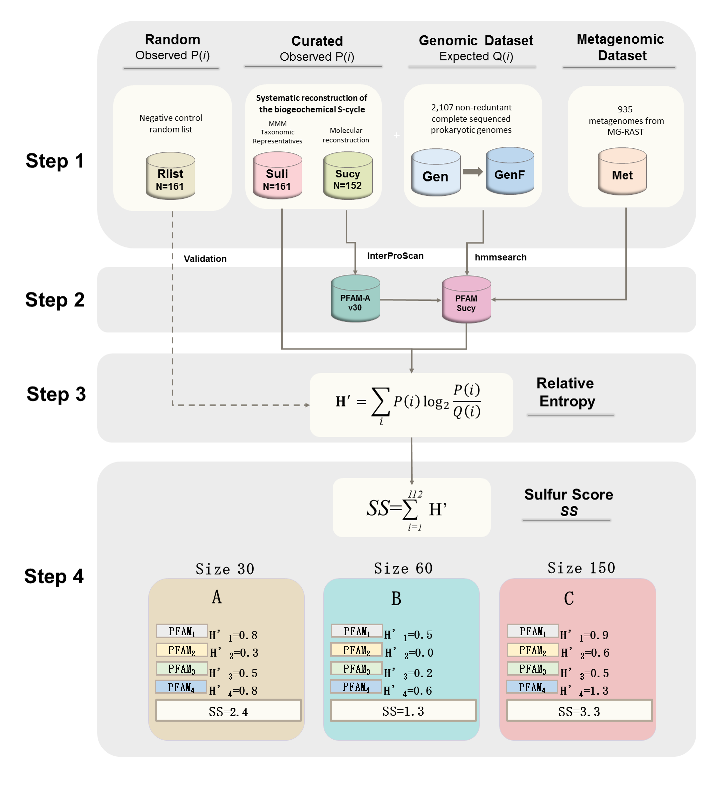
\includegraphics[scale=0.8]{flowchart.png}
    \caption{The MEBS pipeline comprises four steps. Steps 1-3 (\textbf{"advanced mode"}) are required to train an entropy-based classifier, and require expert intervention and data curation (\textbf{step 1}), annotation of Pfam protein domains (\textbf{step 2}) and computing relative entropies of domains annotated in proteins related to the cycle of interest (\textbf{step 3}). Once these steps are completed, the trained model can be used to score arbitrary genomes or metagenomes (\textbf{step 4}, which is called \textbf{"simple mode"}). In the example, the Sulfur Score (SS) is computed for three metegenomic peptide sets with mean fragment sizes of 30, 60 and 150, respectively.}
        \label{fig:pipeline}
\end{figure}

\section{Simple mode}
\label{simple_mod}
Arbitrary FASTA peptide files can be scored by the user. These can be extracted from annotated genomes or metagenomes derived from Microbial Gene Prediction sofware (i.e \texttt{Prodigal}). Alternatively, sequences from \texttt{RefSeq} or \texttt{MG-RAST} databases can be used as well. 

Sample genomes and metagenomes files are provided in folders \verb+test\_genomes/+ and \verb+test\_metagenomes/+, respectively. They can be scored in terms of their \textbf{Sulfur cycle} metabolic machinery with BASH scripts \textit{score\_genomes.sh} and \textit{score\_metagenomes.sh}, as  summarized in Figure \ref{fig:mebs_simple}. These scripts require \verb+hmmsearch+ to be installed.

\begin{figure}[H]
  \centering
    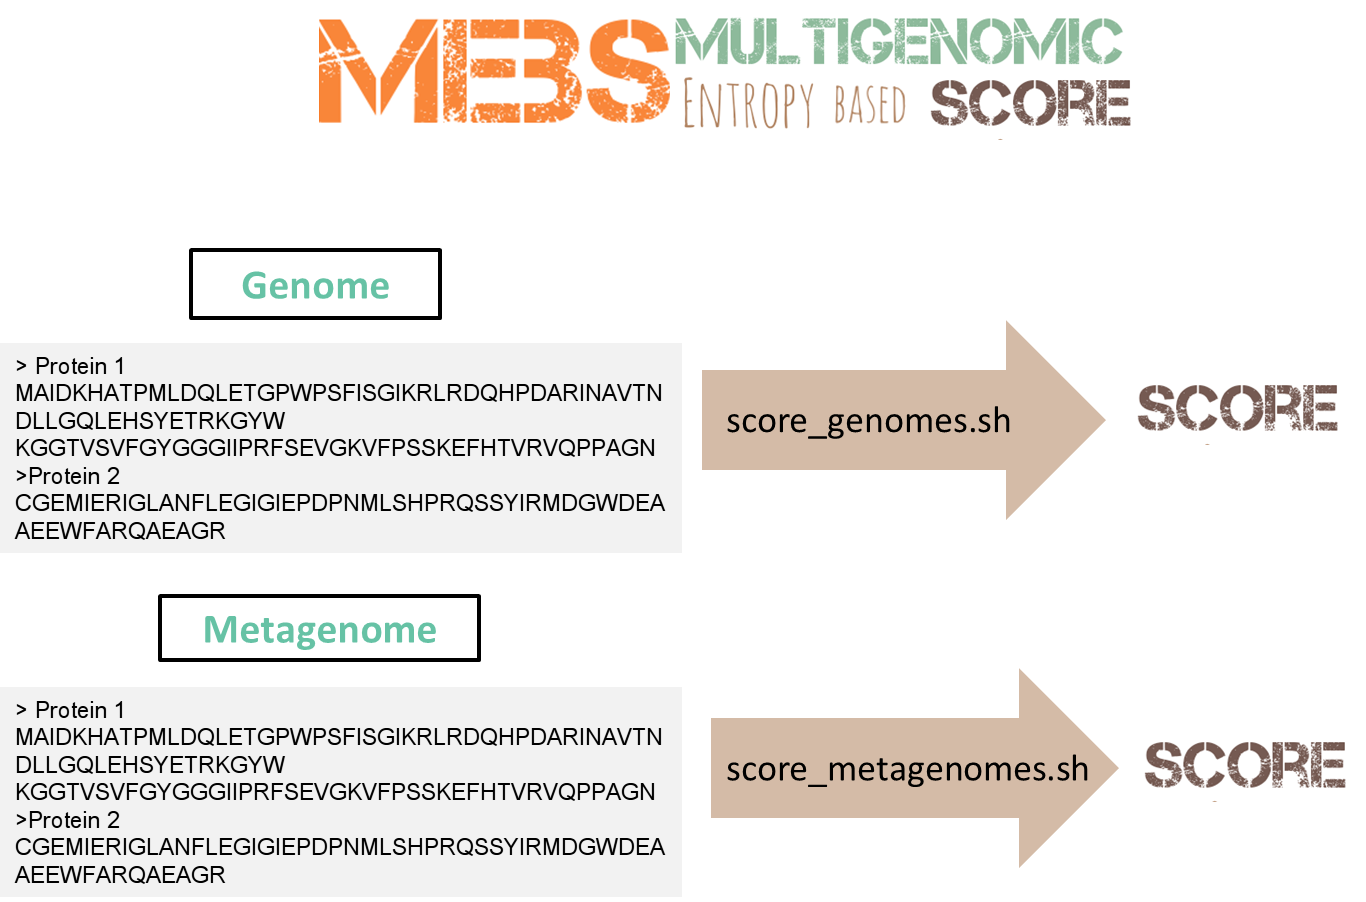
\includegraphics[scale=0.5]{Usage1.png}
    \caption{Running MEBS simple mode}
        \label{fig:mebs_simple}
\end{figure}

More generally, these scripts can be used to analyze a directory containing peptide FASTA files of encoded proteins/fragments with .faa extension. Examples of use would be:

\begin{verbatim}
$ ./score_genomes.sh test_genomes
or
$ ./score_metagenomes.sh test_metagenomes
\end{verbatim}

\section{Advanced mode}

\subsection{Step 1: Databases and manual curation}
\label{stage1}
\subsubsection{Curated input}
The following files must be curated by the user in order to train his/her own data. 
\begin{enumerate}
\label{sucy}
\item  MultiFASTA file with peptide sequences related to the metabolism of
interest. See for instance the contents of the \textbf{Sucy} FASTA file, provided with this software 
(\verb+sulfur_data_test/input_sulfur_data/sucy_database_uniprot.fasta+):
\begin{verbatim}
>sp|Q54506|SAT_RIFPS Sulfate adenylyltransferase OS=Riftia...
MIKPVGSDELKPLFVYDPEEHHKLSHEAESLPSVVISSQGPRVSSMMGAGYFSPAGFMNV
ADAMGAAEKMTLSDGSSSCSVLCLLENTDAIGDAKRIALRDPNVEGNPVLAVMDIEAIEE
VSDEQMAVMTDKVYRTTDMDHIGVKTFNSQGRVAVSGPIQVLNFSYFQADFPDTFRTAVE
IRNEIKEHGWSKVVAFQTRNPMHRAHEELCRMPMESLDADGVVVHMLLGKLKKGDIPAPV
RDAAIRTMAEVYFPPNTVMVTGYGFDMLYAGPREAVLHAYFRQNMGATHFIIGREPPAWV
TTTVPSTPRPSSMTKCQRAPWRSRSSCRPHGLLQEAEQDCDDARRAGSHQGRLRTALRHQ
GREMLGQGIAPPPEFSRPEVAKILMDLLPVHQQLILIWFSGKTRPGVGRWRVFLCAAGAL
WPEAVAVANMEKRSSTG
>tr|O33997|O33997_ALLVI Adenylylsulfate reductase alpha subunit...
MAYKTIIEDGIDVLVVGAGLGGTGAAFEARYWGQDKKIVIAEKANIDRSGAVAQGLYAIN
...
\end{verbatim}

\item List of genomes with know/documented metabolic capabilities. See the example \textbf{Suli} file in \verb+sulfur_data_test/input_sulfur_data/sulfur_list_genomes.txt+: 
\label{suli}
\begin{verbatim}
GCF_000006985.1	Chlorobium tepidum TLS
GCF_000007005.1	Sulfolobus solfataricus P2
GCF_000007305.1	Pyrococcus furiosus DSM 3638
GCF_000008545.1	Thermotoga maritima MSB8
GCF_000008625.1	Aquifex aeolicus VF5
GCF_000008665.1	Archaeoglobus fulgidus DSM 4304
...
\end{verbatim}

%\item FASTA peptide files of annotated genomes or metagenomes. These are the same files used in the simple mode option of \texttt{MEBS}
\end{enumerate}

\subsubsection{Genomic dataset}

In order to benchmark the classifier, we use \texttt{RefSeq} database to obtain  well-annotated, reference genomic prokaryotic sequences. Then, we reduce redundancy using the web-based tool described in \href{http://bioinformatics.oxfordjournals.org/content/early/2013/02/27/bioinformatics.btt064.full}{Moreno-Hagelsieb et al. 2014}.
We conducted the first benchmark of \texttt{MEBS} in 2014, with data from
\texttt{NCBI}, which is provided in \verb+sulfur_data_test/old_data_2014+. We then decided to use \texttt{Refseq}, and a second benchmark was carried out in 2016.

\begin{enumerate}
\label{gen_release}
\item If the user wants to use the same dataset to train his/her own data, it can be downloaded from \href{https://github.com/eead-csic-compbio/metagenome_Pfam_score/releases/tag/gen_2016}{GitHub}. In this case the following steps can be skipped.  

\item  On the contrary, if the user wants to repeat all the steps with the up-to-date contents of Refseq, the following steps are needed. Before you start make sure you have at least of 110Gb of free space in your drive to store the genomic and genomic fragmented datasets. 
\end{enumerate}
 
 \subsubsection{Building your own genomic dataset (Gen)}
 
Visit the \href{http://microbiome.wlu.ca/research/redundancy/redundancy.cgi}{Genome Clusters} server and set the following parameters:
\begin{verbatim}
GSS / DNA Signature = GSSb
GSS threshold = 0.95
DNA-signature threshold = 0.01
Sort by size or overannotation = largest
Results style = simple list
\end{verbatim}

In our Sulfur cycle benchmark, the RefSeq release of August 2016 contained 4085 prokariotic genomes, which were reduced to 2,114 clusters and eventually 2,107 non-redundant genomes. % 7 RefSeq accessions could not be found in the assembly file
Our nr list can be inspected at \verb+sulfur_data_test/Gen/GSSb-0.95.txt+:
\begin{verbatim}
Group 1 GCF_000005825
Group 2 GCF_000005845,GCF_000006925.....
Group 3 GCF_000006175
Group 4 GCF_000006605
Group 5 GCF_000006625,GCF_000019345,GCF_000828735
...
\end{verbatim}

Follow these steps in order to get a multiFASTA file of non-redundant set of genomes.  
\begin{enumerate} 
\item Parse the former list in order to obtain the identifiers of non-redundant
genomes

\begin{verbatim}
$ cd sulfur_data_test/Gen/
$ sed 's/,/\t/g' GSSb-0.95.txt  | sed 's/ /\t/g'  | cut -f 3  > 
list_nr_genomes_21122016.txt
\end{verbatim}

\item Obtain the assembly data from the selected non redundant genomes 
\label{assembly_file}
\begin{verbatim}
$ wget "ftp://ftp.ncbi.nlm.nih.gov/genomes/refseq
/assembly_summary_refseq.txt" 
$ for i in `cat list_nr_genomes_21122016.tx` ; do grep $i 
assembly_summary_refseq.txt >> assembly_refseq.nr2016.txt ; done
\end{verbatim}

\item Get the download links 

\begin{verbatim}
$ less assembly_refseq.nr2016.txt | cut -f 20 | sed 's/$/\/*.faa.gz/g' 
> assembly_refseq.nr2016.download.txt
\end{verbatim}

\item Download the genomes in \verb+faa+ format  

\begin{verbatim}
$ wget -i assembly_refseq.nr2016.download.txt
$ gunzip *.gz 
\end{verbatim}
\item Before generate a multiFASTA file, it is important to change the headers of all the genomes for latter purposes, described in section \ref{step2}

\begin{verbatim}
$ for i in *.faa ; do perl -lne 'if(/^>(\S+)/){ print ">$1 [$ARGV]"} 
else{ print }' $i > $i.named.faa; done
\end{verbatim}
\item The previous command will change the headers from
\begin{verbatim}
>WP_003320558.1 MULTISPECIES: ATP-binding protein 
[Bacillus]
MNEQIQAYAKRLKLSWIRENFNQIEAETNEEYLLKLFEKEVQNREERKVNLLLSQ
AQLPKTGSTPFQWEHIQIPQGIERT
\end{verbatim}
to this 
\begin{verbatim}
>WP_003320558.1 [GCF_000005825.2_ASM582v2_protein.faa]
MNEQIQAYAKRLKLSWIRENFNQIEAETNEEYLLKLFEKEVQNREERKVNLLLSQ
AQLPKTGSTPFQWEHIQIPQGIERT
\end{verbatim}

\item  Generate the multiFASTA file 

\begin{verbatim}
$ cat *.named.faa > genomes_refseq_nr_22122016.faa
\end{verbatim}

\item Generate one-line multiFASTA file using the following perl snippet

\begin{verbatim}
$ perl -lne 'if(/^(>.*)/){ $head=$1 } else { $fa{$head} .= $_ } END{ 
foreach $s (sort(keys(%fa))){ print "$s\n$fa{$s}\n" }}' 
genomes_refseq_nr_22122016.faa > genomes_refseq_nr_22122016.1.faa & 
\end{verbatim}

\end{enumerate}

\subsubsection{Building your own Genomic fragmented dataset (GenF)}

Using the multiFASTA file containing the non-redundant genomes, then the genomic fragmented set can be generated using script \textit{get\_protein\_fragments.pl}.

Depending on the Mean Size Length (\texttt{MSL}) observed in the fragmented metagenomic dataset, the the Genomic fragmented dataset is generated. We use seven categories to fragment the Genomic dataset: 30, 60, 100, 150, 200, 250 and 300. These sizes were choosen due to the observed bins in the Metagenomic dataset, see details in section \ref{msl}. In order to see the help page you can type:

\begin{verbatim}
$ perl scripts/get_protein_fragments.pl 

Program to produce random fragments of proteins in input file 
with size and coverage set by user.
usage: get_protein_fragments.pl [options] 
 -help    brief help message
  -inFASTA    input file with protein sequences in FASTA format
 -outFASTA    output file with protein fragments in FASTA format
  -size    desired size for produced random fragments    
  (integer, default 100)
  -cover    desired protein coverage of produced fragment (integer, default 1) 
\end{verbatim}

We can now loop along the desired fragment sizes:

\begin{verbatim}
$ for i in 30 60 100 150 200 250 
perl get_protein_fragments.pl -inFASTA genomes_refseq_nr_21122016.1.faa \
	-oUTFASTA genomes_refseq_nr_21122016_size${i}_cover10.faa -size $i -cover 10 ;
done 
\end{verbatim}

Then create a new directory containing the \textit{in silico} sheared FASTA files. 
\begin{verbatim}
$ mkdir sulfur_data_test/GenF && mv *cover* sulfur_data_test/GenF
\end{verbatim}
\label{directory_genF}
Using the above commands, the following files should be generated (Table \ref{sizes}).  

\begin{table}[H]
\centering
\caption{Description of the genomic and genomic fragmented datasets}
\label{sizes}
\begin{tabular}{@{}lll@{}}
\toprule
Details             & File name                                           & Size File \\ \midrule
nr-genomes          & genomes\_refseq\_nr\_22122016.1.faa                 & 2.7G      \\
nr-genomes size 30  & genomes\_refseq\_nr\_21122016\_size30\_cover10.faa  & 7.8 G     \\
nr-genomes size 60  & genomes\_refseq\_nr\_21122016\_size60\_cover10.faa  & 9.8 G     \\
nr-genomes size 100 & genomes\_refseq\_nr\_21122016\_size100\_cover10.faa & 13 G      \\
nr-genomes size 150 & genomes\_refseq\_nr\_21122016\_size150\_cover10.faa & 16 G      \\
nr-genomes size 200 & genomes\_refseq\_nr\_21122016\_size200\_cover10.faa & 18 G      \\
nr-genomes size 250 & genomes\_refseq\_nr\_21122016\_size200\_cover10.faa & 20 G      \\
nr-genomessize 300  & genomes\_refseq\_nr\_21122016\_size200\_cover10.faa & 22 G      \\ \bottomrule
\end{tabular}
\end{table}

\subsubsection{Metagenomic dataset}

If you want to train your classifier  using public available metagenomes, you can
use the following commands to download them from \texttt{MG-RAST} server version 3.6. Otherwise, if
you have your own data, skip this step, and compute the Mean Size Length of your  metagenomes (see section \ref{msl}).

\subsubsection{Building your own metagenomic dataset}

Generate a list of metagenomes of interest. We selected only those metagenomes that meet the following
conditions:
\begin{enumerate}
\item Public and available metagenomes
\item Available metadata associated 
\item Environmental samples (isolated from defined environments o features:
rivers, soil, biofilms, etc), discarding the microbiome associated metagenomes
(i.e human, cow, chicken)
\item We also included 35 private metagenomes unpublished derived from
sediment, water and microbial mats from Cuatro Cienegas Coahuila (De Anda, in
progress).
\end{enumerate}

Using the above mentioned conditions, a total of 935 id-numbers were
saved in list format

See the example file \verb+sulfur_data_test/Met/id_metagenomes.txt+: 
\begin{verbatim} 
4524971.3
4451035.3
4557986.3
4441021.3
...
\end{verbatim}

\subsubsection{Considerations}
\begin{enumerate}
\item If you decide to use the data in the  \textit{id\_metagenomes.txt} file, please be aware that this process will take several hours, and at least 500 Gb of drive space. 
\item Otherwise you can change the id-numbers from those of your interest.  
\item Make sure you are inside folder \verb+sulfur_data_test/Met/+

\item Get the corresponding encoded protein sequences using the  \href{http://api.metagenomics.anl.gov/api.html}{MG-RAST API}. 
\begin{verbatim}
$ for line in  `cat id_metagenomes.txt` ; do wget
"http://api.metagenomics.anl.gov/1/download/mgm$line?file=350.1" -O $line ;
done

#Check the files 

$ head 4524971.3
>FA4S SCL02FZQ74_1_237_-
LGRPIDIESLDVSFWGGLGVVLGNVVISNPEDMPGDTLMVAKEI
DVKLQLWPLLSSEVRADRFIINDPTI
>FA4SSCL02ILJM5_1_200_-
YIYLTLVEFKGQAAGLRERESIQHFQWSDKQVSKKEGSFGVDHI
WYLQGIFMCSSIQKDYPKIK

#Make sure that all the files were downloaded correctly 

$find -empty | wc
\end{verbatim}
\item  Make sure you are located in the same directory containing the peptides from the downloaded metagenomes and compute the Mean Size Length (\texttt{MSL}) of each metagenome  using the following one-line perl script:

\label{msl}
\begin{verbatim}
$ for FILE in *; do perl -lne 'if(/^(>.*)/){$h=$1}else{$fa{$h}.=$_} 
END{ foreach $h (keys(%fa)){$m+=length($fa{$h})}; 
printf("%1.0f\t",$m/scalar(keys(%fa))) }' $FILE; echo $FILE; done > 
MSL.tab
\end{verbatim}
\item See the example of the MSL output from all the 935 metagenomes 

\begin{verbatim}
$ head  sulfur_data_test/Met/MSL.tab 

52	4524971.3
79	4451035.3
75	4441022.3
\end{verbatim}
\item Plot the MSL sizes \ref{fig:msl_metagenomes}
\begin{verbatim}
Open R from the terminal 
$ R 
> data<-read.table("sulfur_data_test/Met/MSL.tab", header=F, sep="\t")
> pdf("hist.msl.pdf")
> hist(data$V1,main= "MSL metagenomic dataset",xlab= "MSL in aa")
> dev.off()
> quit()
$ evince hist.msl.pdf  & 
\end{verbatim}
\end{enumerate}
  \begin{figure}[H]
  \centering
    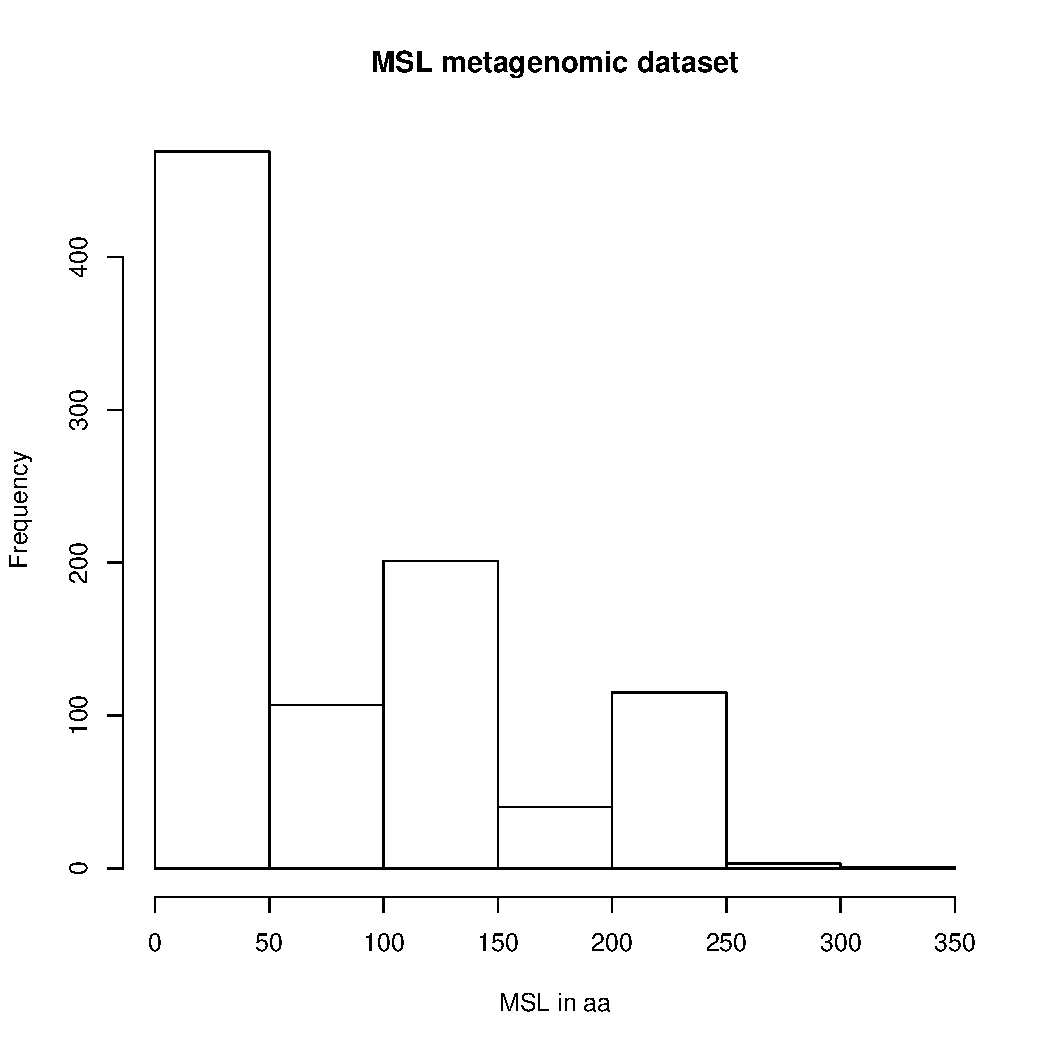
\includegraphics[width=50mm, scale=0.5]{hist.pdf}
    \caption{MSL histogram of the metagenomic dataset }
        \label{fig:msl_metagenomes}
\end{figure}


\subsubsection{Building your own random dataset}

\label{building_random}
The random dataset consist of arbitrary number of lists containing random genomes not particularly enriched in the metabolism of interest. For this purposes, consider the same number of genomes from your input list. First you need to know how many genomes are you given as input, as described in section \ref{suli} and then shuffle the assembly file from \texttt{RefSeq} to get random accession numbers.
\begin{verbatim}
#1. First create a new directory containing all the list to be generated 
$ mkdir random samples 

#2. Count the number of genomes in your input list 
$ num=`less sulfur_data_test/input_sulfur_data/  sulfur_list_genomes.txt | \
wc -l`

#3. Create 1000 list of random accession numbers  
$ for ((i=1;i<1001;i+=1)); do cat sulfur_data_test/Gen/assembly_refseq.nr2016.txt \
| cut -f 1,8 | shuf -n $num  > random_samples/random$i.txt  ; done
\end{verbatim}

The random created lists, will be used in section \ref{random_entropy}

\subsection{STEP 2: Domain annotation}
\label{step2}

\begin{enumerate}
\item Annotate the domain composition of your input proteins (See  example in section \ref{sucy}) using \texttt{InterproScan}  and the current release of \texttt{PfamA} database (updated December 2016)

\begin{verbatim}
#Run interproscan 

$ interproscan.sh -appl PfamA-30.0 \
-i  sulfur_data_test/input_sulfur_data/sucy_database_uniprot.fasta 
\ -f tsv -pa  -iprlookupD
\end{verbatim}

\item  Check the output example, using  following the output information of
\href{https://github.com/ebi-pf-team/interproscan/wiki/InterProScan5OutputFormats}{InterproScan}

\begin{verbatim}
$ less -S sulfur_data_test/sucy_database_uniprot.fasta.tsv
P38038  fb5aec671520cf6aab02a5a3862c2aeb        599     Pfam    PF00258 ..
P38038  fb5aec671520cf6aab02a5a3862c2aeb        599     Pfam    PF00175 ..
\end{verbatim}

\item In order to get the family domains of the input  proteins, make sure that you have the current release of Pfam database. Usually is installed with Interproscan. You also can get the current Pfam release using the following command line. 
\begin{verbatim}
$ wget ftp://ftp.ebi.ac.uk/pub/databases/Pfam/current_release/Pfam-A.hmm.gz
gunzip Pfam-A.hmm.gz

\end{verbatim}

\item Get the specific \texttt{Pfam} domain accession numbers of the input proteins. Use the output file from \texttt{InterproScan}
\begin{verbatim}
$ cut -f 4,5 \
sulfur_data_test/sucy_database_uniprot.fasta.tsv >id_interpro.txt 
\end{verbatim}

\item Obtain the specific markov models of the input proteins.Run the script \textit{extract\_hmms.pl}. 
The latter use as input the  id\_interpro.txt  and the  PfamA.hmm. Make sure
you have those files in the same directory. And the names are exactly the same,
otherwise the script will not work.

\begin{verbatim}
$ perl scripts/extract_hmms.pl 

# Pfam
# hmms = 112 #pfam version 30. 
\end{verbatim}
This will generate an output file named '\verb+my_Pfam.hmm+. We have compressed the file, which is provided precomputed at \verb+sulfur_data_tes/my_Pfam.hmm.bz2+

Note that Superfamily and TIGRFAM HMMs can also be used, but are commented out in the script since in our tests they produced huge outfiles (SF) or largely redundant with Pfam (TIGR).

\item Annotate Pfam domains in the "omic"-data sets using HMMER.

\label{hmmsearch-gen}
\subsubsection*{Pfam annotation in the multifasta file of non-redundant genomes }
If you build your own non redundant dataset, change the <*.faa> input file by your file name. Otherwise, you could use file containing 2107 genomes as described above in section  \ref{gen_release}
\begin{verbatim}
$ hmmsearch --cut_ga -o /dev/null  --tblout 
genomes_refseq_nr_22122016.fa.pf.tab  
my_Pfam.hmm genomes_refseq_nr_22122016.1.faa  & 
\end{verbatim}

Optionally, you can compute  hmmsearch for each genome separately, in order to calculate their Score as explained in detail in \ref{Step4} 

\subsubsection*{Pfam annotation in the metagenomic dataset}  
\begin{verbatim}

$ for i in sulfur_data_test/Met/* ; do \ 
hmmsearch --cut_ga -o /dev/null --tblout \
$i.out.hmmsearch.tab my_Pfam.hmm  $i; done &
\end{verbatim}
\end{enumerate}


\subsection{STEP 3: Relative Entropy}
\label{Step 3}

We used a derivative of the Kullback-Leibler divergence, also known as relative entropy, to measure the difference between two probability
distributions P(i) and Q(i). See \ref{eq:eq1}

\begin{equation}
  \label{eq:eq1}
  H' = P(i)log_2\frac{P(i)}{Q(i)}
\end{equation}

In this context, P(i) 
represents the total number of occurrences of protein 
family i in sulfur-related genomes (observed frequency), 
while Q(i) represents the total number of occurrences of 
that family in the genomic dataset (expected frequency). The relative entropy H', in bits, captures the extent to which a family informs 
specifically about sulfur metabolism. H' values that are 
close to 1 correspond to the most informative families 
(enriched among sulfur-related genomes), whereas low H'
values (close to zero) describe non-informative families. 
Negative values correspond to protein families observed 
less than expected

\subsubsection*{Requirements to compute relative entropies}
\label{entropies_requirements}
\begin{enumerate}
\item  A hmmsearch TSV outfile with the results of scanning 
a collection of Pfam domais against  a large set of(non-
redundant) genomes (output from hmmsearch in the omic 
datasets ) described in section \ref{hmmsearch-gen}. 
We provided the outfile derived from the results of scanning 
the 112 Sulfur related models  against the 2,107 non redundant genomes described in section \ref{hmmsearch-gen}
Download the file from the   \href{https://github.com/eead-csic-compbio/metagenome_Pfam_score/releases/tag/HMM_gen}{GitHub-release}

\item A list of selected accessions of genomes interest to compute entropy see example file  \verb+sulfur_data_test/input_sulfur_data/sulfur_list_genomes.txt+, described in section \ref{suli}

\item An optional list of \texttt{RefSeq} assembly annotations to print scientific names
instead of accession codes. See example file
\verb+sulfur_data_test/Gen/assembly_refseq.nr2016.txt+ described in section \ref{assembly_file}
\end{enumerate}

\subsubsection*{Computing the relative entropy in the genomic dataset} 

The entropies matrices precomputed for the genomic (Gen) and genomic fragmented (GenF) are provided in the 
\verb+sulfur_data_test/entropies_matrix+  directory.  
We provided the data to compute the matrices for the Gen dataset.For space reasons GenF is not provide, but it can be easily generated as explained in previous sections \ref{directory_genF}. 
The entropies matrices are obtained with the script \textit{entropy.pl}.
Firs Run the script help:
\begin{verbatim}
$ perl scripts/entropy.pl : usage: scripts/entropy.pl 
<pfam_hmmsearch.tab> <accession list (ie Suli)> <RefSeq 
list, optional>
\end{verbatim}
Create a directory containing the obtained matrices 
\begin{verbatim}
$ mkdir entropies_matrix
\end{verbatim}
Obtain the entropy matrix from the Gen dataset (Real size).
\begin{verbatim}
$ perl scripts/entropy.pl genomes_refseq_nr_22122016.1.faa.out.hmmsearch.tab 
sulfur_data_test/input_sulfur_data/sulfur_list_genomes.txt
sulfur_data_test/Gen/assembly_refseq.nr2016.txt > 
entropies_matrix/genomes_refseq_nr_22122016.fa.pf.tab.csv
\end{verbatim}

After computing the relative entropies from your own data, you will get the following files: 
\begin{enumerate}
\item  A matrix of occurrence of Pfam domains across genomes
\item Entropy estimates of each scanned Pfam domain with respect to the selected accessions
\end{enumerate}

\subsubsection*{Observing the distribution of the relative entropies}

In order to plot the results obtained with the \textit{entropy.pl} script, the
following scripts are needed:   

\begin{enumerate}

\item  \textit{entropies.py}: The first script requires all the matrix that
contains the relative entropies computed in the genomic and genomic 
fragmented data-set (sizes 30, 60, 100, 150, 200, 250, 
300). The matrix are located in entropies\_matrix 
directory. The scripts  returns a tabular list of the 
entropies. Make sure that the names of the matrix in csv 
format follow this pattern \'\_size([0-9]+)\_\', otherwise 
the script cannot be computed. Besides, all the files need to 
have the same number of domains (profiles) in the same column 
order. This script assumes that these considerations are true, 
so it cannot find errors in the input files format.
\begin{verbatim}
$ python3 scripts/extract_entropies.py entropies_matrix/
\end{verbatim}
The latter script will generate the text file \verb+entropies_matrix_entropies.tab+
\begin{verbatim}
        real    30      60      100     150     200 ...    
PF00005 -0.001  0.001   -0.001  -0.001  -0.001  -0.001 ...
PF00009 -0.001  -0.014  -0.001  -0.001  -0.001  -0.001 ...
PF00034 -0.119  -0.195  -0.183  -0.153  -0.115  -0.106 ...
\end{verbatim}

\item \textit{plot\_entropy.py}: In order to observe the results of the latter
tabular file, this scripts will generate 5 different plots:
\begin{verbatim}
Usage:
        $ python3 plot_entropy.py data.tab [random perc5] [random perc95]

Run the script
       $ python3 plot_entropy.py entropies_matrix_entropies.tab
\end{verbatim}

After running the script, the following figures are generated: 
\begin{enumerate}

\item \textbf{entropies\_matrix\_entropies.tab\_bar.png.} Barplot of the
distribution of each Pfam relative entropy, in the different genomic fragmented
sizes. At the top of the figure are the  Pfam's with highest values, and the
bottom are the lowest entropies values . (Figure \ref{fig:barplot})

 \begin{figure}[H]
  \centering
    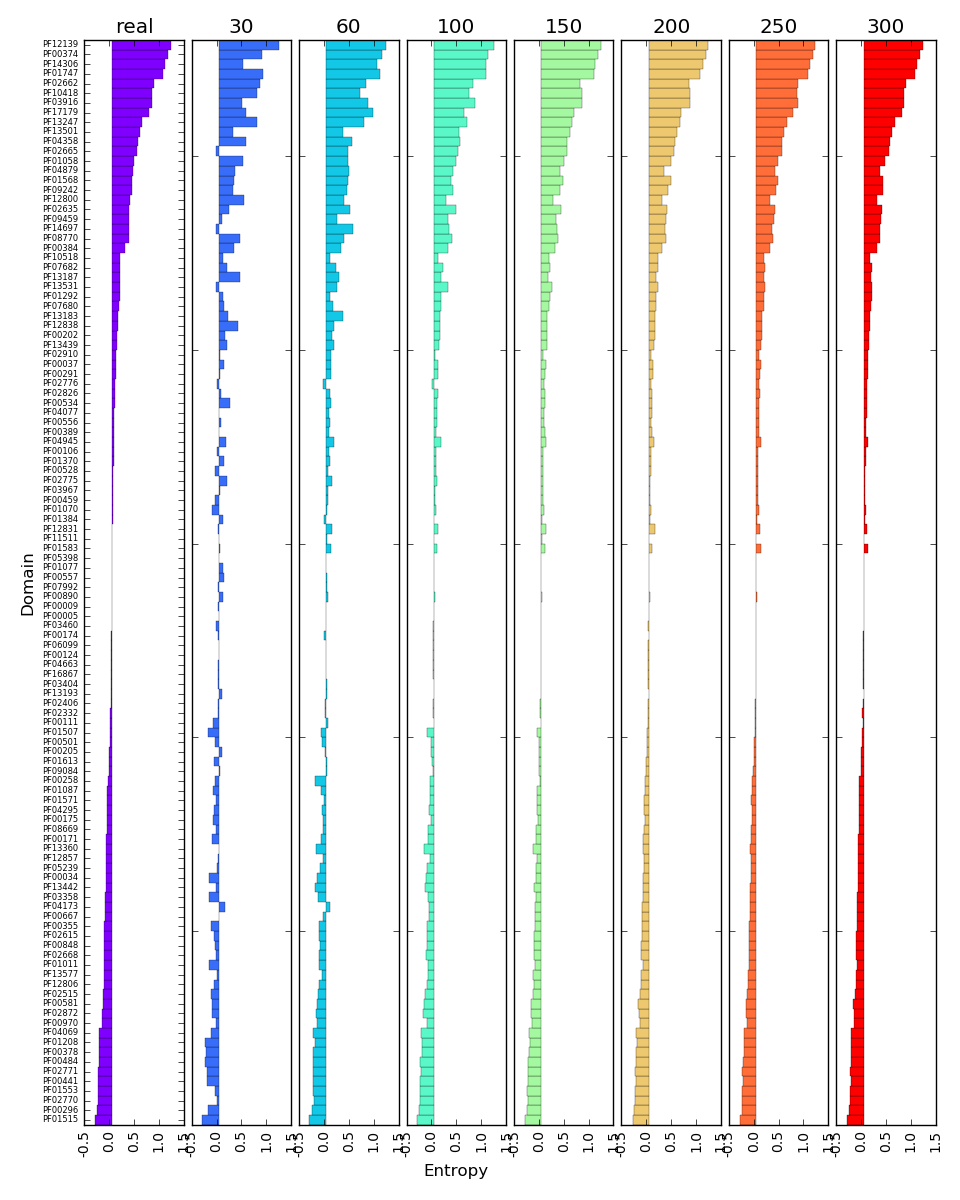
\includegraphics[width=450px]{entropies_matrix_entropies_tab_bar.png}
    \caption{Distribution of relative entropies of Pfam domains in Gen and GenF.}
        \label{fig:barplot}
\end{figure}

\item \textbf{entropies\_matrix\_entropies.tab\_hmap.png}. Heatmap of the
distribution of each Pfam relative entropy, in the different genomic fragmented
sizes. Red values are the highest entropies and blue values the lowest. (Figure
\ref{fig:heatmap})
 \begin{figure}[H]
  \centering
    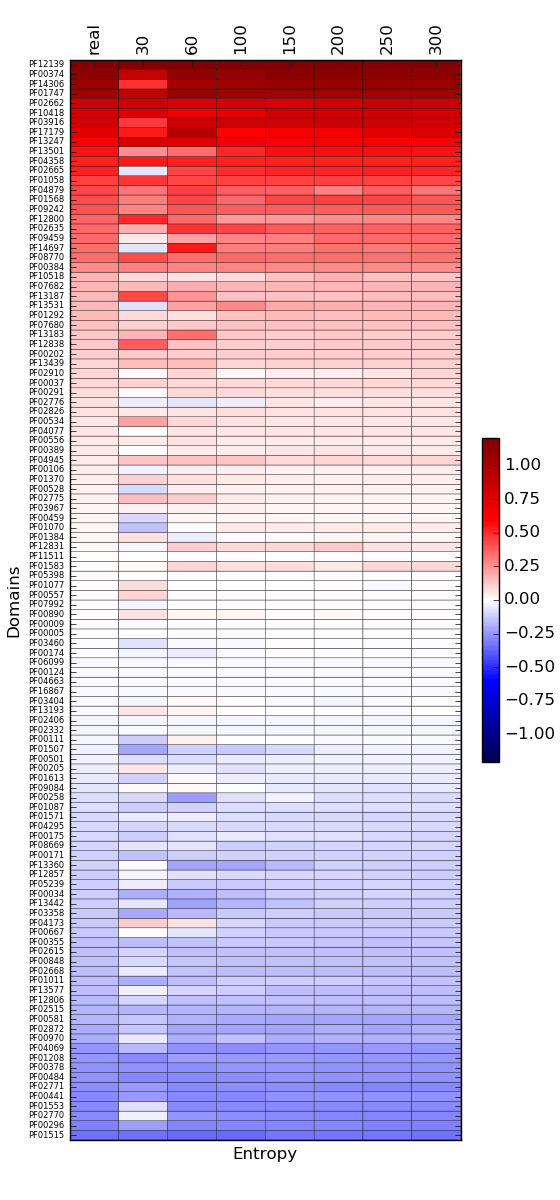
\includegraphics[width=320px, scale =0.9]{entropies_matrix_entropies_tab_hmap.png}
    \caption{Distribution of relative entropies of Pfam domains in Gen and GenF.}
        \label{fig:heatmap}
\end{figure}

\item \textbf{entropies\_matrix\_entropies.tab\_scatter.png}. Scatter plot
showing the mean dispersion of each  Pfam H' (x axis),versus the standard
deviation of the values obtained in the genomic fragmented dataset (y axis). In
this sense the low standard deviation indicates that the H' values are similar
across several datasets of variable sizes, which is useful in the metagenomic
dataset. In this sense, the H' of this specific Pfam's, are not affected by the
size of the metagenome (either read peptides of 30 aa or 300). In the other
hand, high standard deviation indicates that H' is affected by the size. In
this way, high H', and low standard deviation, points the most informative
Pfam's that could be used as molecular marker genes in metagenomes of variable
sizes. (Figure \ref{fig:scatterplot}) 
 \begin{figure}[H]
  \centering
    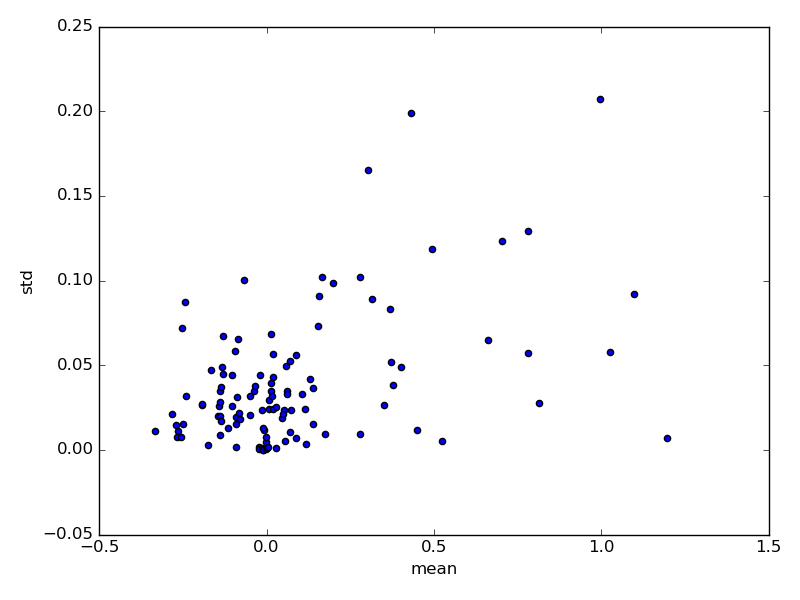
\includegraphics[width=300px, scale =0.5]{entropies_matrix_entropies_tab_scatter.png}
    \caption{Dispersion of Pfam entropies.}
        \label{fig:scatterplot}
\end{figure}


\item \textbf{entropies\_matrix\_entropies.tab\_entropy\_hist.png}. Histograms
of the distribution of the H' in the different genomic fragmented sizes.
(Figure \ref{fig:histogram})

\begin{figure}[H]
  \centering
    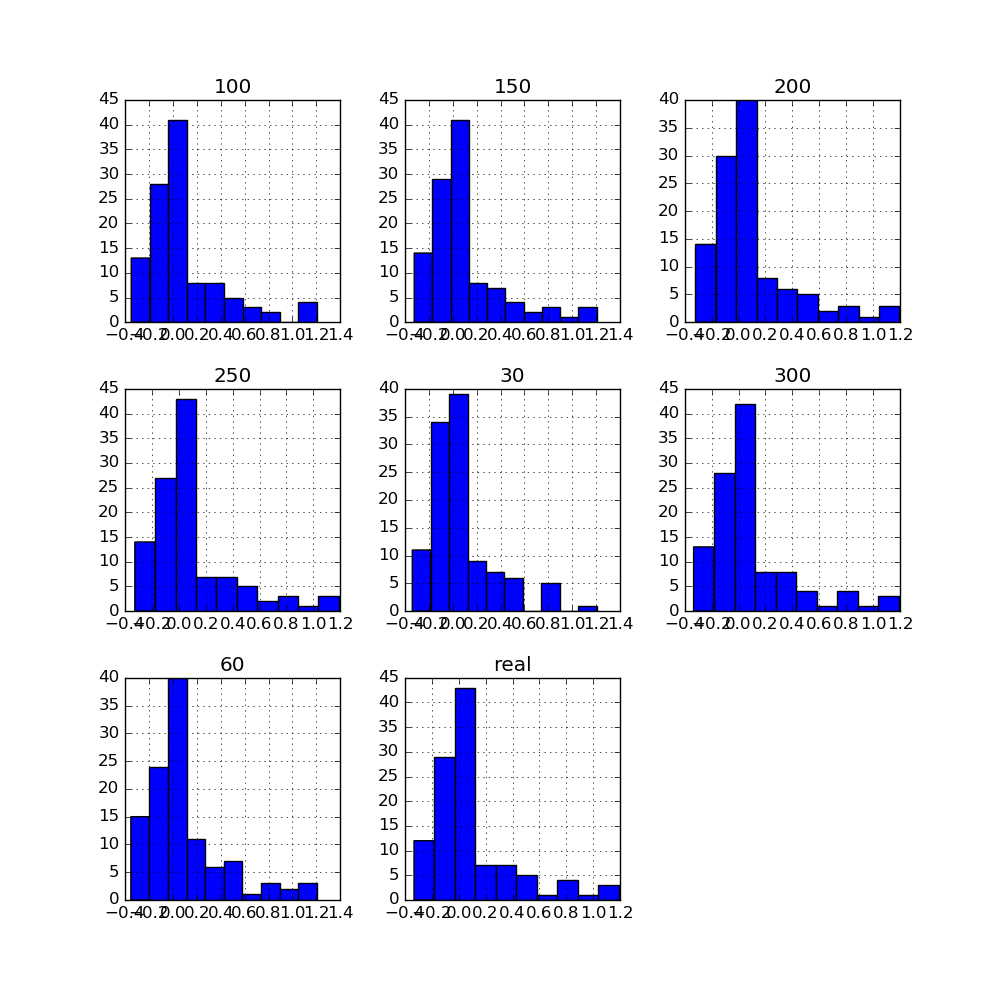
\includegraphics[width=350px, scale =0.5]{entropies_matrix_entropies_tab_entropy_hist.png}
    \caption{Distribution of Pfam entropies in Gen and GenF datasets.}
        \label{fig:histogram}
\end{figure}

\item \textbf{entropies\_matrix\_entropies.tab\_differential.png}.

Entropy difference of each Pfam H' with respect to real, in order to observe
the degree of change from the previous one. The differential was calculate
along the MSL 

                      \textbf{          $x_i - x_{i-1}$.}

The data was normalized with respect to real values, then the differential was
plotted according to each size (MSL). The highest entropy difference with
respect to real values is obteined in sizes of 30 and 60, indicating that above
this values, the H' of each Pfam are maintained across several datasets of
variable sizes (>60). (Figure \ref{fig:differential})

 \begin{figure}[H]
  \centering
    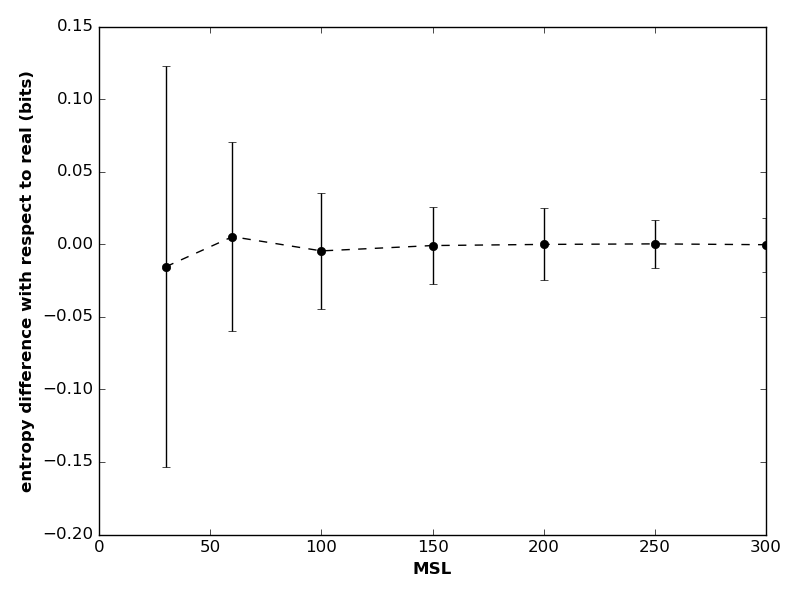
\includegraphics[width=300px, scale =0.5]{entropies_matrix_entropies_tab_differential.png}
    \caption{Differential plot }
        \label{fig:differential}
\end{figure}

\item \textbf{entropies\_matrix\_entropies.tab\_prof\_box.png}.Boxplot the
distribution of each Pfam relative entropy, in the different genomic fragmented
sizes. Middle blue line indicates cero values. Black lines indicates the
percentile data  (5\% and 95\%) obtained obtained in the random test. (Figure
\ref{fig:boxplot}). See further details in Random entropies.  

\begin{figure}[H]
  \centering
    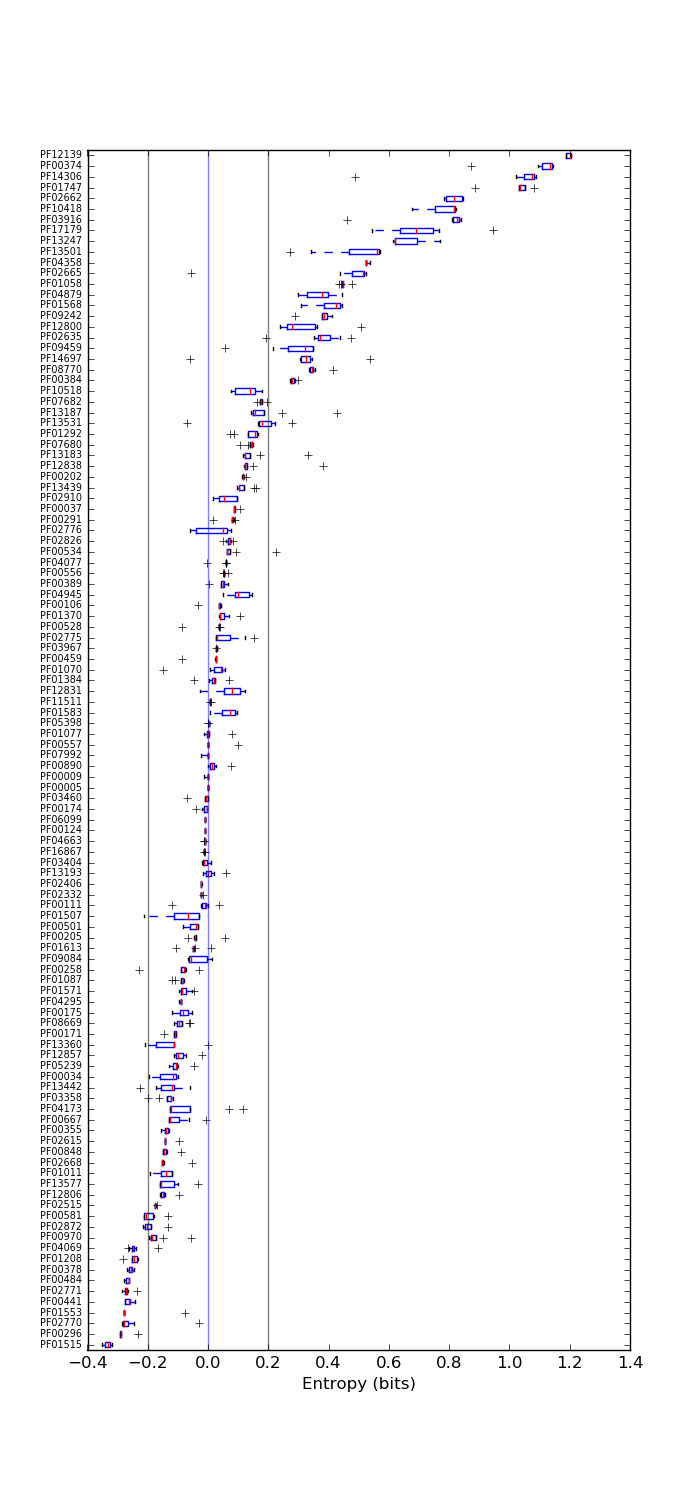
\includegraphics[width=250px, scale =0.5]{entropies_matrix_entropies_tab_prof_box.png}
    \caption{Boxplot distribution of Pfam relative entropies in Gen and GenF}
        \label{fig:boxplot}
\end{figure}

\label{random_entropy}
\subsection{STEP 3: Relative entropy of random datasets}
Generate the entropies from each of the the random list computed in section \ref{building_random}. 
\begin{enumerate}
\item First, compute the random entropies from Gen dataset
\begin{verbatim}
$ for i in random_samples/*.txt; do perl scripts/entropy.pl 
genomes_refseq_nr_22122016.1.faa.out.hmmsearch.tab $i > $i.csv;
done 
\end{verbatim}
\item Then use the GenF to compute the random entropies considering fragmented sizes
You can either save these command lines into a bash script. 
\begin{verbatim}
#!/bin bash
for msl in 30 60 100 150 200 250 300 
do  
for file in random_samples/*.txt; do perl scripts/entropy.pl 
genomes_refseq_nr_22122016_size"${msl}"_cover10.faa.out.hmmsearch.tab  
$file > $file.$msl.csv
 done
done
echo "Done, please check the csv matrices in random_samples"  

\end{verbatim}
\item Extract the entropies values of all the 8,000 matrices, and get a tabular format file of each Pfam and the corresponding  H' value on each test (1..100). Use the script \textit{extract\_random\_entropies.pl}
\begin{verbatim}

perl ../scripts/extract_random_entropies.pl -matrixdir 
random_samples/

# extract_random_entropies.pl call:
# -matrixdir random_samples

# merged file of MSL=real (replicates=1000, random_real.real.tab)
\end{verbatim}
\item Generate a new folder and move all the generated files 
\begin{verbatim}
mkdir tab_files_random && mv *.tab tab_files_random  
\end{verbatim}
\item Plot the tabular files output using the following script
\begin{verbatim}
python3 scripts/plot_random_entropies.py random_real.real.tab 
\end{verbatim}
\item Using the above mentioned script, we obtained both: 1) the percentile data of
all the tabular files computed for each size (MSL) (Table \ref{percent}), and
2) the boxplot distribution of each  Pfam H' value in the the random
%test(Figure \ref{fig:cutoff_random}).
See the complete description of the output files.
\begin{verbatim}.
1) Percentile distribution at 5% and 95%  of each Pfam H',  in the 
1000 random matrices, for example:

PF13501  5-percentile= -0.049  95-percentile= 0.077
PF13531  5-percentile= -0.058  95-percentile= 0.058

2) The total min 5-percentile and max 95-percentile 
# min  5-percentile= -0.091
# max 95-percentile= 0.101

3)Boxplot distribution of each Pfam H', indicating the lines of the 
max an min percentile distribution. 
\end{verbatim}
\end{enumerate}
After running the entropy random test using the Sulfur cyle data, you will get the following percentile distribution of the Gen and GenF.  \ref{percent}, 

\begin{table}[H]
\centering
\caption{min 5 and max 95 percentile distribution of Pfam's H' in each MSL}
\label{percent}
\begin{tabular}{@{}ccc@{}}
\toprule
MSL  & 5 percentile & 95 percentile \\ \midrule
Real & -0.091       & 0.101         \\
30   & -0.086       & 0.105         \\
60   & -0.09        & 0.105         \\
100  & -0.088       & 0.1           \\
150  & -0.09        & 0.103         \\
200  & -0.089       & 0.105         \\
250  & -0.09        & 0.106         \\
300  & -0.09        & 0.1             \\ \bottomrule
\end{tabular}
\end{table}



\end{enumerate}
\end{enumerate}

\subsection{STEP 4: Entropy Score and interpretation}
\label{Step4}
\subsubsection{Requirements}
Due to the variation in peptide size within metagenomic datasets (see
Figure \ref{fig:msl_metagenomes}, it would be computationally expensive to fragment the genomic datasets in all the observed sizes. Therefore, we chose to fragment them according to the observed sizes/bins in the histogram (see (Figure \ref{fig:msl_metagenomes}):
30,60,100,150,200,250 and 300. Taking this into
account, we propose a range of $\pm 15$ aminoacid residues above or below the size to
compute the Score. Accordingly, entropy scores for a metagenome of MSL of 40 would be computed using pre-computed entropies of the genomic fragmented (GenF) dataset
of size 30. See Table \ref{MSL-input}

\begin{table}[H]
\centering
\caption{MSL selection of input metagenome}
\label{MSL-input}
\begin{tabular}{@{}lll@{}}
\toprule
Details             & GenF size & MSL     \\ \midrule
nr-genomes size 30  & 30        & 0-45    \\
nr-genomes size 60  & 60        & 46-80   \\
nr-genomes size 100 & 100       & 81-125  \\
nr-genomes size 150 & 150       & 126-175 \\
nr-genomes size 200 & 200       & 176-225 \\
nr-genomes size 250 & 250       & 226-275 \\
nr-genomessize 300  & 300       & 276-300 \\ \bottomrule
\end{tabular}
\end{table}

%If you want to compute the Score selecting entropies of a certain VALUE (H'>=1), you can select this option, however  the higher the number chosen for the entropy, the less informative the SS will be. Therefore, we do not recommend the entropy cut-off. 

\subsubsection{Computing the Entropy Score}
\label{entropy_score}

The final Entropy Score, Sulfur Score in the case of the Sulfur cycle, can be computed by calling script \textit{pfam\_score.pl}, located in the scripts directory
\begin{verbatim}
perl scripts/pfam_score.pl
usage: pfam_score.pl [options] 

-help             brief help message
-input            input file with HMM matches created by 
                  hmmsearch, tbl format
-size             desired size for produced random 
                  fragments    (integer, default 100)
-bzip             input file is bzip2-compressed
-matrixdir        directory containing hmm matrices from 
                  fragments of variable size (string, 
                  default /data/matrix)
-minentropy       min relative entropy of HMMs to be considered (float)
-keggmap          file with HMM to KEGG mappings
-pathway          comma-separated pathway numbers from -keggmap 
                  file to consider only member HMMs  (string, by default 
                  all pathways are used, requires           -keggmap)
\end{verbatim}

This script was implicitely invoked by the score scripts presented in the "simple mode" section (\ref{simple_mod}). Here we provide some examples of usage: 
\begin{enumerate}

\item If you want to compute the Sulfur score for a new genome using the pre-computed entropy matrices for the Sulfur cycle using, please use the following command line:
\begin{verbatim}
$  perl scripts/pfam_score.pl -input test_genomes/Enterococcus_durans.faa \
  -matrixdir  sulfur_data_test/entropies_matrix -size 500 
\end{verbatim}
Note that we specified \verb+-size 500+ in the command line, \textbf{which is the way to tell the script that real, complete sequences are to be used}. 

%even though we are computing the Score in a full sequenced-genome which lack of the fragmentary nature observed in the metagenomic data. The reason why we specified this number is very simple. The \textit{pfam\_score.pl} script, use the entropy matrix file and choose the appropriate entropy value according to the selected input size. Therefore, the appropriate value would be "REAL", however due to practical reasons, the script finds the appropriate size inside the file name. Therefore is important to conserve the same pattern file name, located in \verb+sulfur_data_test/entropies_matrix+ The only requirement is to rename the file name: \verb+genomes_refseq_nr_22122016.fa.pf.tab.csv+
%with an arbitrary size name, in this case we choose 500, but any other number can be used. 
%\verb+genomes_refseq_nr_22122016_size500_cover10.faa.out.hmmsearch.tab.csv+
%Both files are provided are provided in the %\verb+sulfur_data_test/entropies_matrix+, directory. And they are exactly the same files but with different name. \textit{This step need be improved in the newer versions of }\texttt{MEBS}

\item In case you wish to compute the Entropy Score of a metagenome dataset, you must first estimate MSL in order to select the appropriate precomputed Pfam entropies. 

\begin{enumerate}
\item Run the following command to obtain the MSL of your input metagenome. Note that backslashes must be removed:  
 
 \begin{verbatim}
$ perl -lne 'if(/^(>.*)/){$h=$1}else{$fa{$h}.=$_} END{ foreach \
$h (keys(%fa)){$m+=length($fa{$h})};\
printf("MSL = %1.0f\n",$m/scalar(keys(%fa))) }'\ 
test_metagenomes/4440966.3_metagenome.faa > 
4440966.3_metagenome.faa.msl 
# MSL = 175
\end{verbatim}

\item Using the obtained MSL, you can either choose the appropiated GenF entropies according to the Table \ref{MSL-input}, or you can use the following script to choose the size automatically. 

\begin{verbatim}
$ perl -lne 'BEGIN{@bins=(30,60,100,150,200,250,300);\
  @th=(45,80,125,175,225,275,300)} if(/^MSL = (\S+)/){ $msl=$1; \  
  foreach $i (0 .. $#th){ \ 
  if($msl<=$th[$i]){ print "genF = $bins[$i]"; exit } } }'\
  4440966.3_metagenome.faa.msl .msl \ >    
  4440966.3_metagenome.faa.msl .genF
  cat 4440966.3_metagenome.faa.msl.genF
\end{verbatim}

\item Save the GenF size into a variable  
  
  \begin{verbatim}
$ genF=`perl -lne 'if(/genF = (\S+)/){ print $1 }'\
  4440966.3_metagenome.faa.msl.genF`
  \end{verbatim}
    
\item Run the Entropy Score
    \begin{verbatim}
$ perl scripts/pfam_score.pl -input \ 
4440966.3_metagenome.faa.out.hmmsearch.tab  \
-size $genF -matrixdir sulfur_data_test/entropies_matrix > \
4440966.3_metagenome.faa.out.hmmsearch.tab.score
\end{verbatim}
\end{enumerate}
\end{enumerate}

As mentioned above, the \texttt{BASH} scripts \verb+score_genomes.sh+ and \verb+score_metagenomes.sh+  read an input directory containing multiFASTA peptide sequences and compute the score using the \textit{pfam\_score.pl} script.

%\begin{verbatim}
%$ ./score_genomes.sh test_genomes
%or
%$ ./score_metagenomes.sh test_metagenomes
%\end{verbatim}

%If you are analyzing hundreds of genomes or metagenomes, use this simple %comand line to get your scores in CSV file.   
%\begin{verbatim}
%grep "Pfam entropy score:" *.score | sed 's/:/\t/g' > 
%total.scores.csv 
%\end{verbatim}

\end{document}
